\documentclass{ximera}

%% You can put user macros here
%% However, you cannot make new environments

\listfiles

\graphicspath{{./}{firstExample/}{secondExample/}}

\usepackage{tikz}
\usepackage{tkz-euclide}
\usepackage{tikz-3dplot}
\usepackage{tikz-cd}
\usetikzlibrary{shapes.geometric}
\usetikzlibrary{arrows}
\usetikzlibrary{decorations.pathmorphing,patterns}
\usetkzobj{all}
\pgfplotsset{compat=1.13} % prevents compile error.

\renewcommand{\vec}[1]{\mathbf{#1}}
\newcommand{\RR}{\mathbb{R}}
\newcommand{\dfn}{\textit}
\newcommand{\dotp}{\cdot}
\newcommand{\id}{\text{id}}
\newcommand\norm[1]{\left\lVert#1\right\rVert}
 
\newtheorem{general}{Generalization}
\newtheorem{initprob}{Exploration Problem}

\tikzstyle geometryDiagrams=[ultra thick,color=blue!50!black]

\usepackage{mathtools}

\title{Motion Under A Central Force}%\label{Module 7-ADEF}


\begin{document}

\begin{abstract}

\end{abstract}

\maketitle

\section*{Motion Under A Central Force}

We'll now study the motion of a object moving under the influence
of a \textit{central force}; that is, a force whose magnitude at any
point $P$ other than the origin depends only on the distance from
$P$ to the origin, and whose direction at $P$ is parallel to the line
connecting $P$ and the origin, as indicated in
the figure below for the case where the direction of the force
at every point is toward the origin.

\begin{image}
 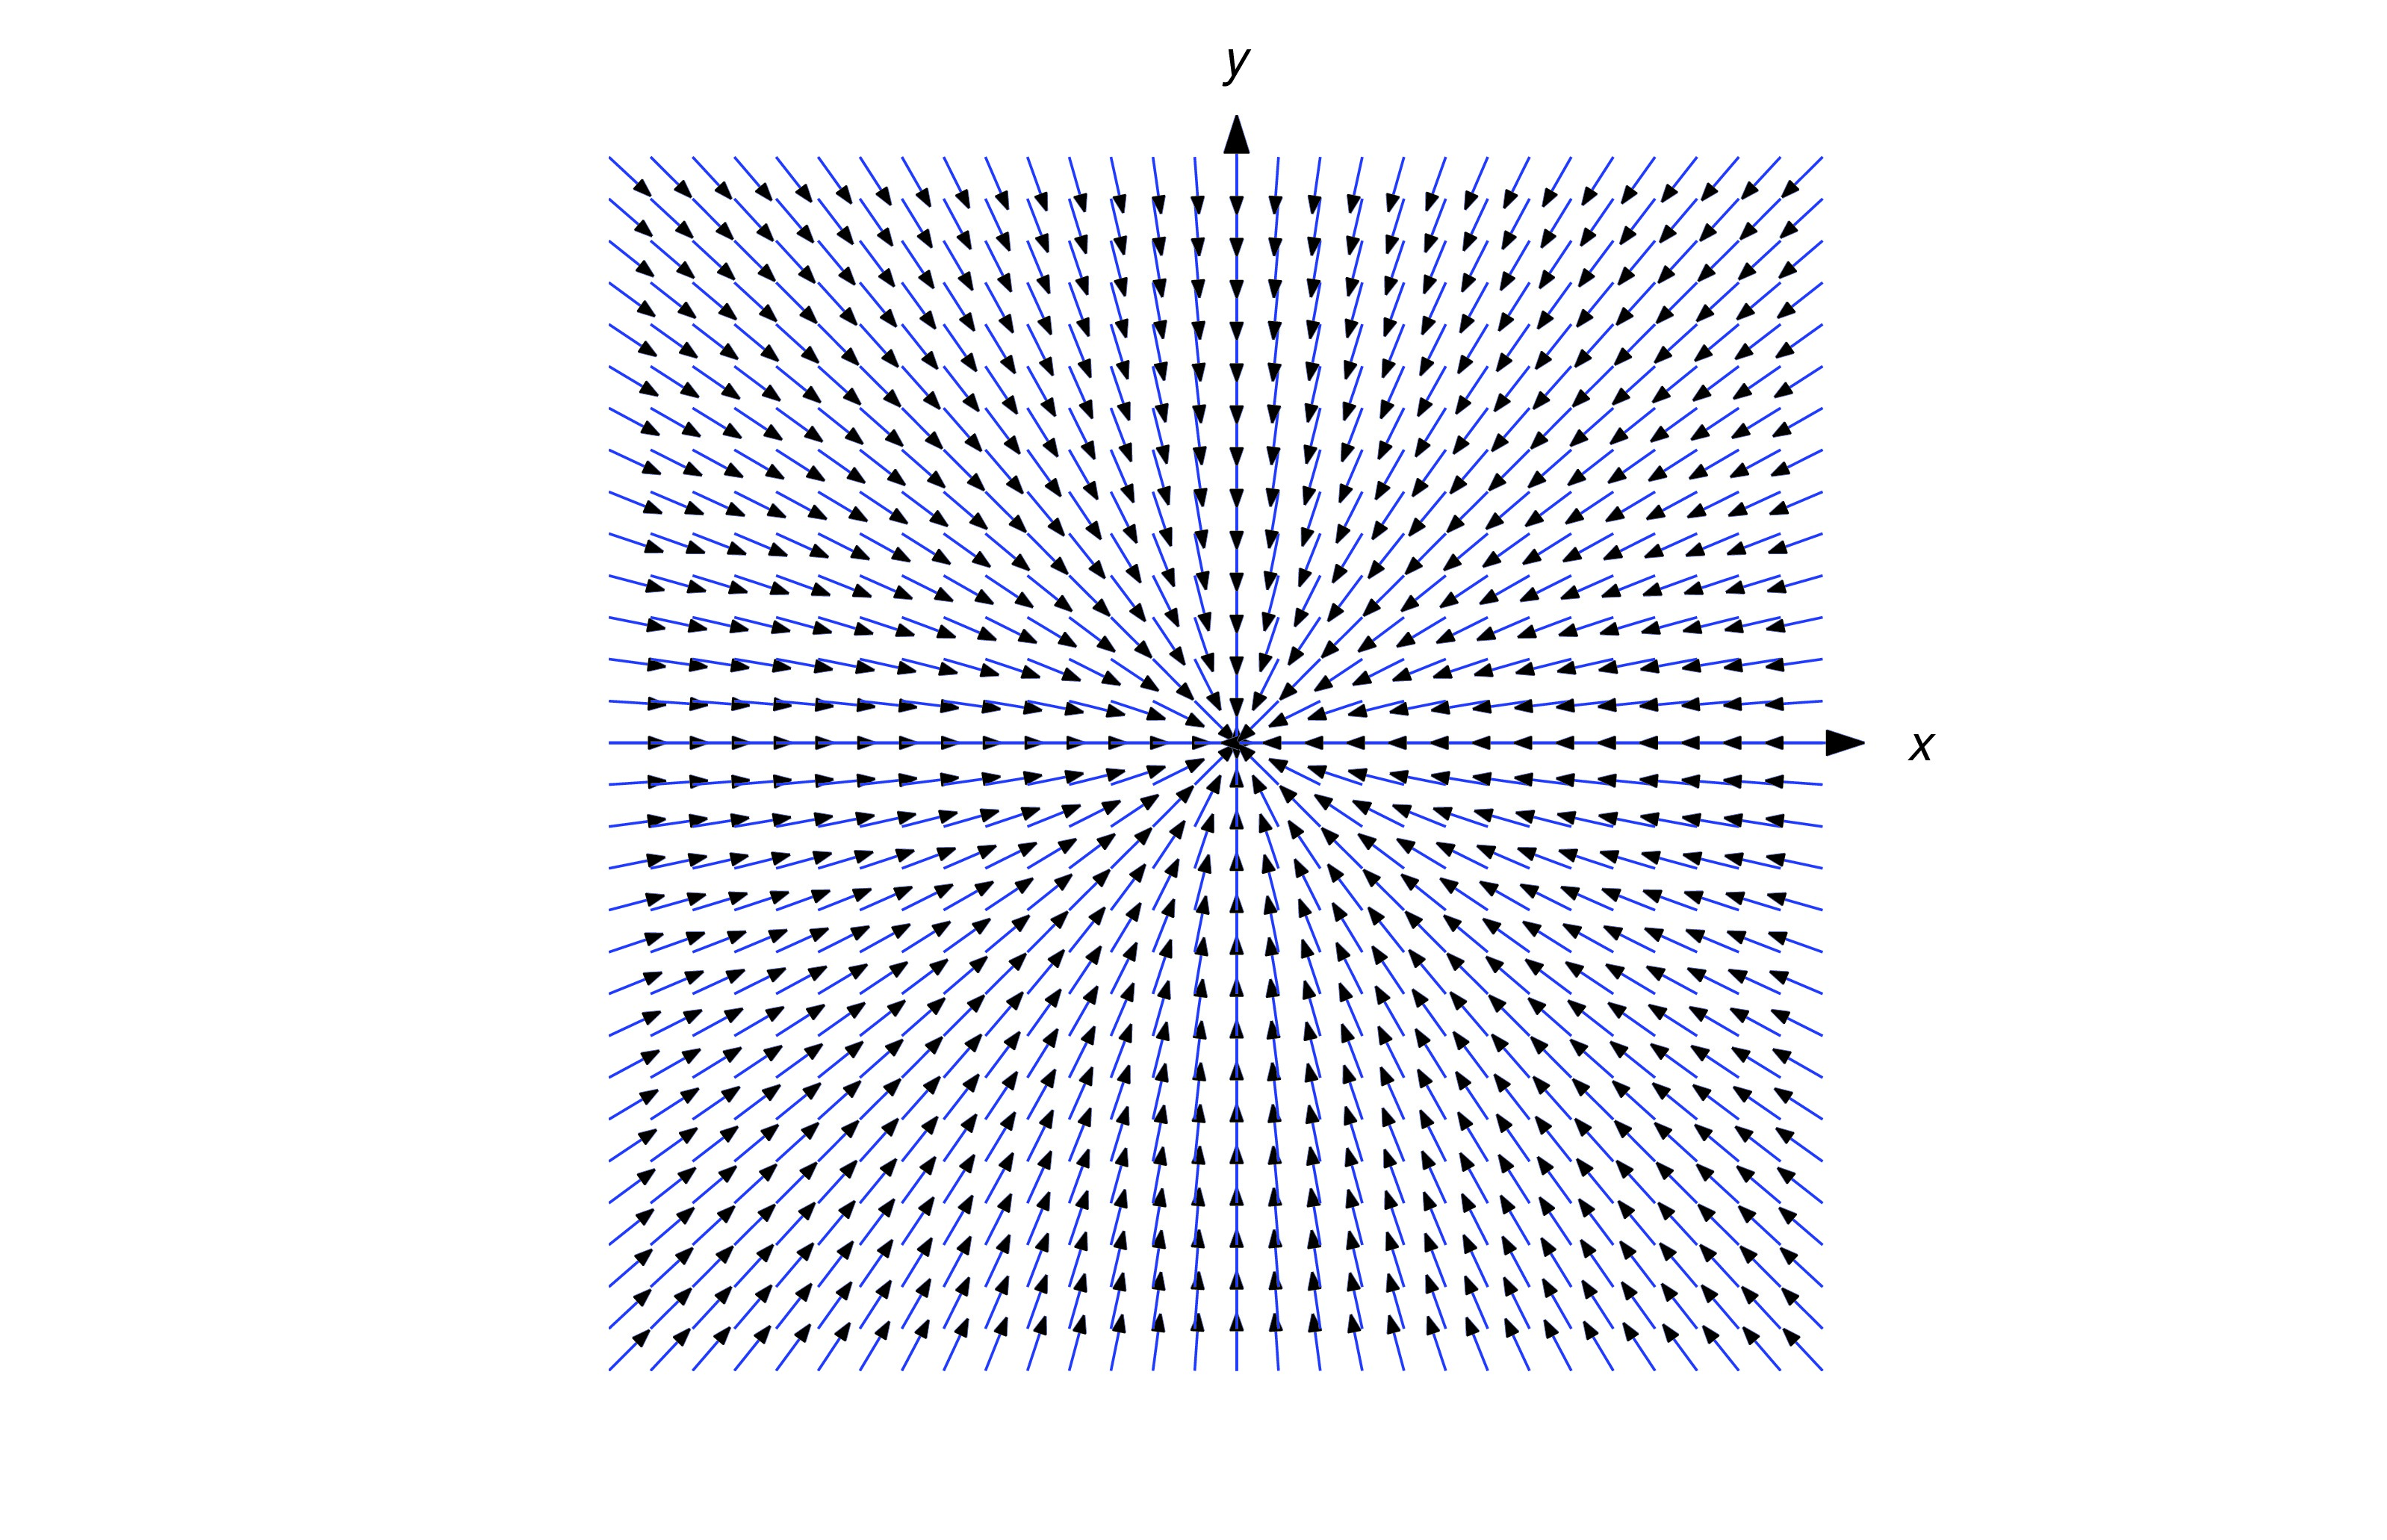
\includegraphics[height=1.5in]{fig060401.jpg}
 \end{image}

 Gravitational forces are central
forces;   for example, as mentioned in Section~4.3, if we
assume that Earth is a perfect sphere with constant mass density then
Newton's law of gravitation asserts that the force exerted on an
object by Earth's gravitational field is proportional to the mass of
the object and inversely proportional to the square of its distance
from the center of Earth, which we take to be the origin.

If the initial position and velocity vectors of an object moving under
a central force are parallel, then the subsequent motion is along the
line from the origin to the initial position. Here we'll assume that
the initial position and velocity vectors are not parallel;   in this
case the subsequent motion is in the plane determined by them. For
convenience we take this to be the $xy$-plane. We'll
consider
the problem of determining the curve traversed by the object. We call
this curve the \textit{orbit}.


We can represent a central force in terms of polar coordinates
$$
x=r\cos\theta,\quad y=r\sin\theta
$$
 as
$$
\vec{F}(r,\theta)=f(r)(\cos\theta\,\vec{i}+\sin\theta\,\vec{j}).
$$
We assume that $f$ is continuous for all $r>0$. The magnitude of $\vec{F}$ at $(x,y)=(r\cos\theta,r\sin\theta)$ is $|f(r)|$, so it depends
only on the distance $r$ from the point to the origin   the direction
of $\vec{F}$ is from the point to the origin if $f(r)<0$, or from the
origin to the point if $f(r)>0$. We'll show that the orbit of an
object with mass $m$ moving under this force is given by
$$
r(\theta)=\frac{1}{u(\theta)},
$$
where $u$  is solution of the differential equation
\begin{equation} \label{eq:6.4.1}
 \frac{d^2u}{d\theta^2}+u=-\frac{1}{mh^2u^2}f(1/u),
\end{equation}
and $h$ is a constant defined below.



Newton's second law of motion ($\vec{F}=m\vec{a}$) says that the polar
coordinates
$r=r(t)$ and $\theta=\theta(t)$ of
the particle  satisfy the vector differential equation
\begin{equation} \label{eq:6.4.2}
m(r\cos\theta\,\vec{i}+r\sin\theta\,\vec{j})''=
f(r)(\cos\theta\,\vec{i}+\sin\theta\,\vec{j}).
\end{equation}
To deal with this equation we introduce  the unit vectors
$$
\vec{e}_1=\cos\theta\,\vec{i}+\sin\theta\,\vec{j}
\quad\mbox{and}\quad
\vec{e}_2=-\sin\theta\,\vec{i}+\cos\theta\,\vec{j}.
$$
Note that   $\vec{e}_1$ points in the
direction of increasing $r$ and $\vec{e}_2$ points in the
direction of increasing $\theta$.  (See the figure below)

\begin{image}
 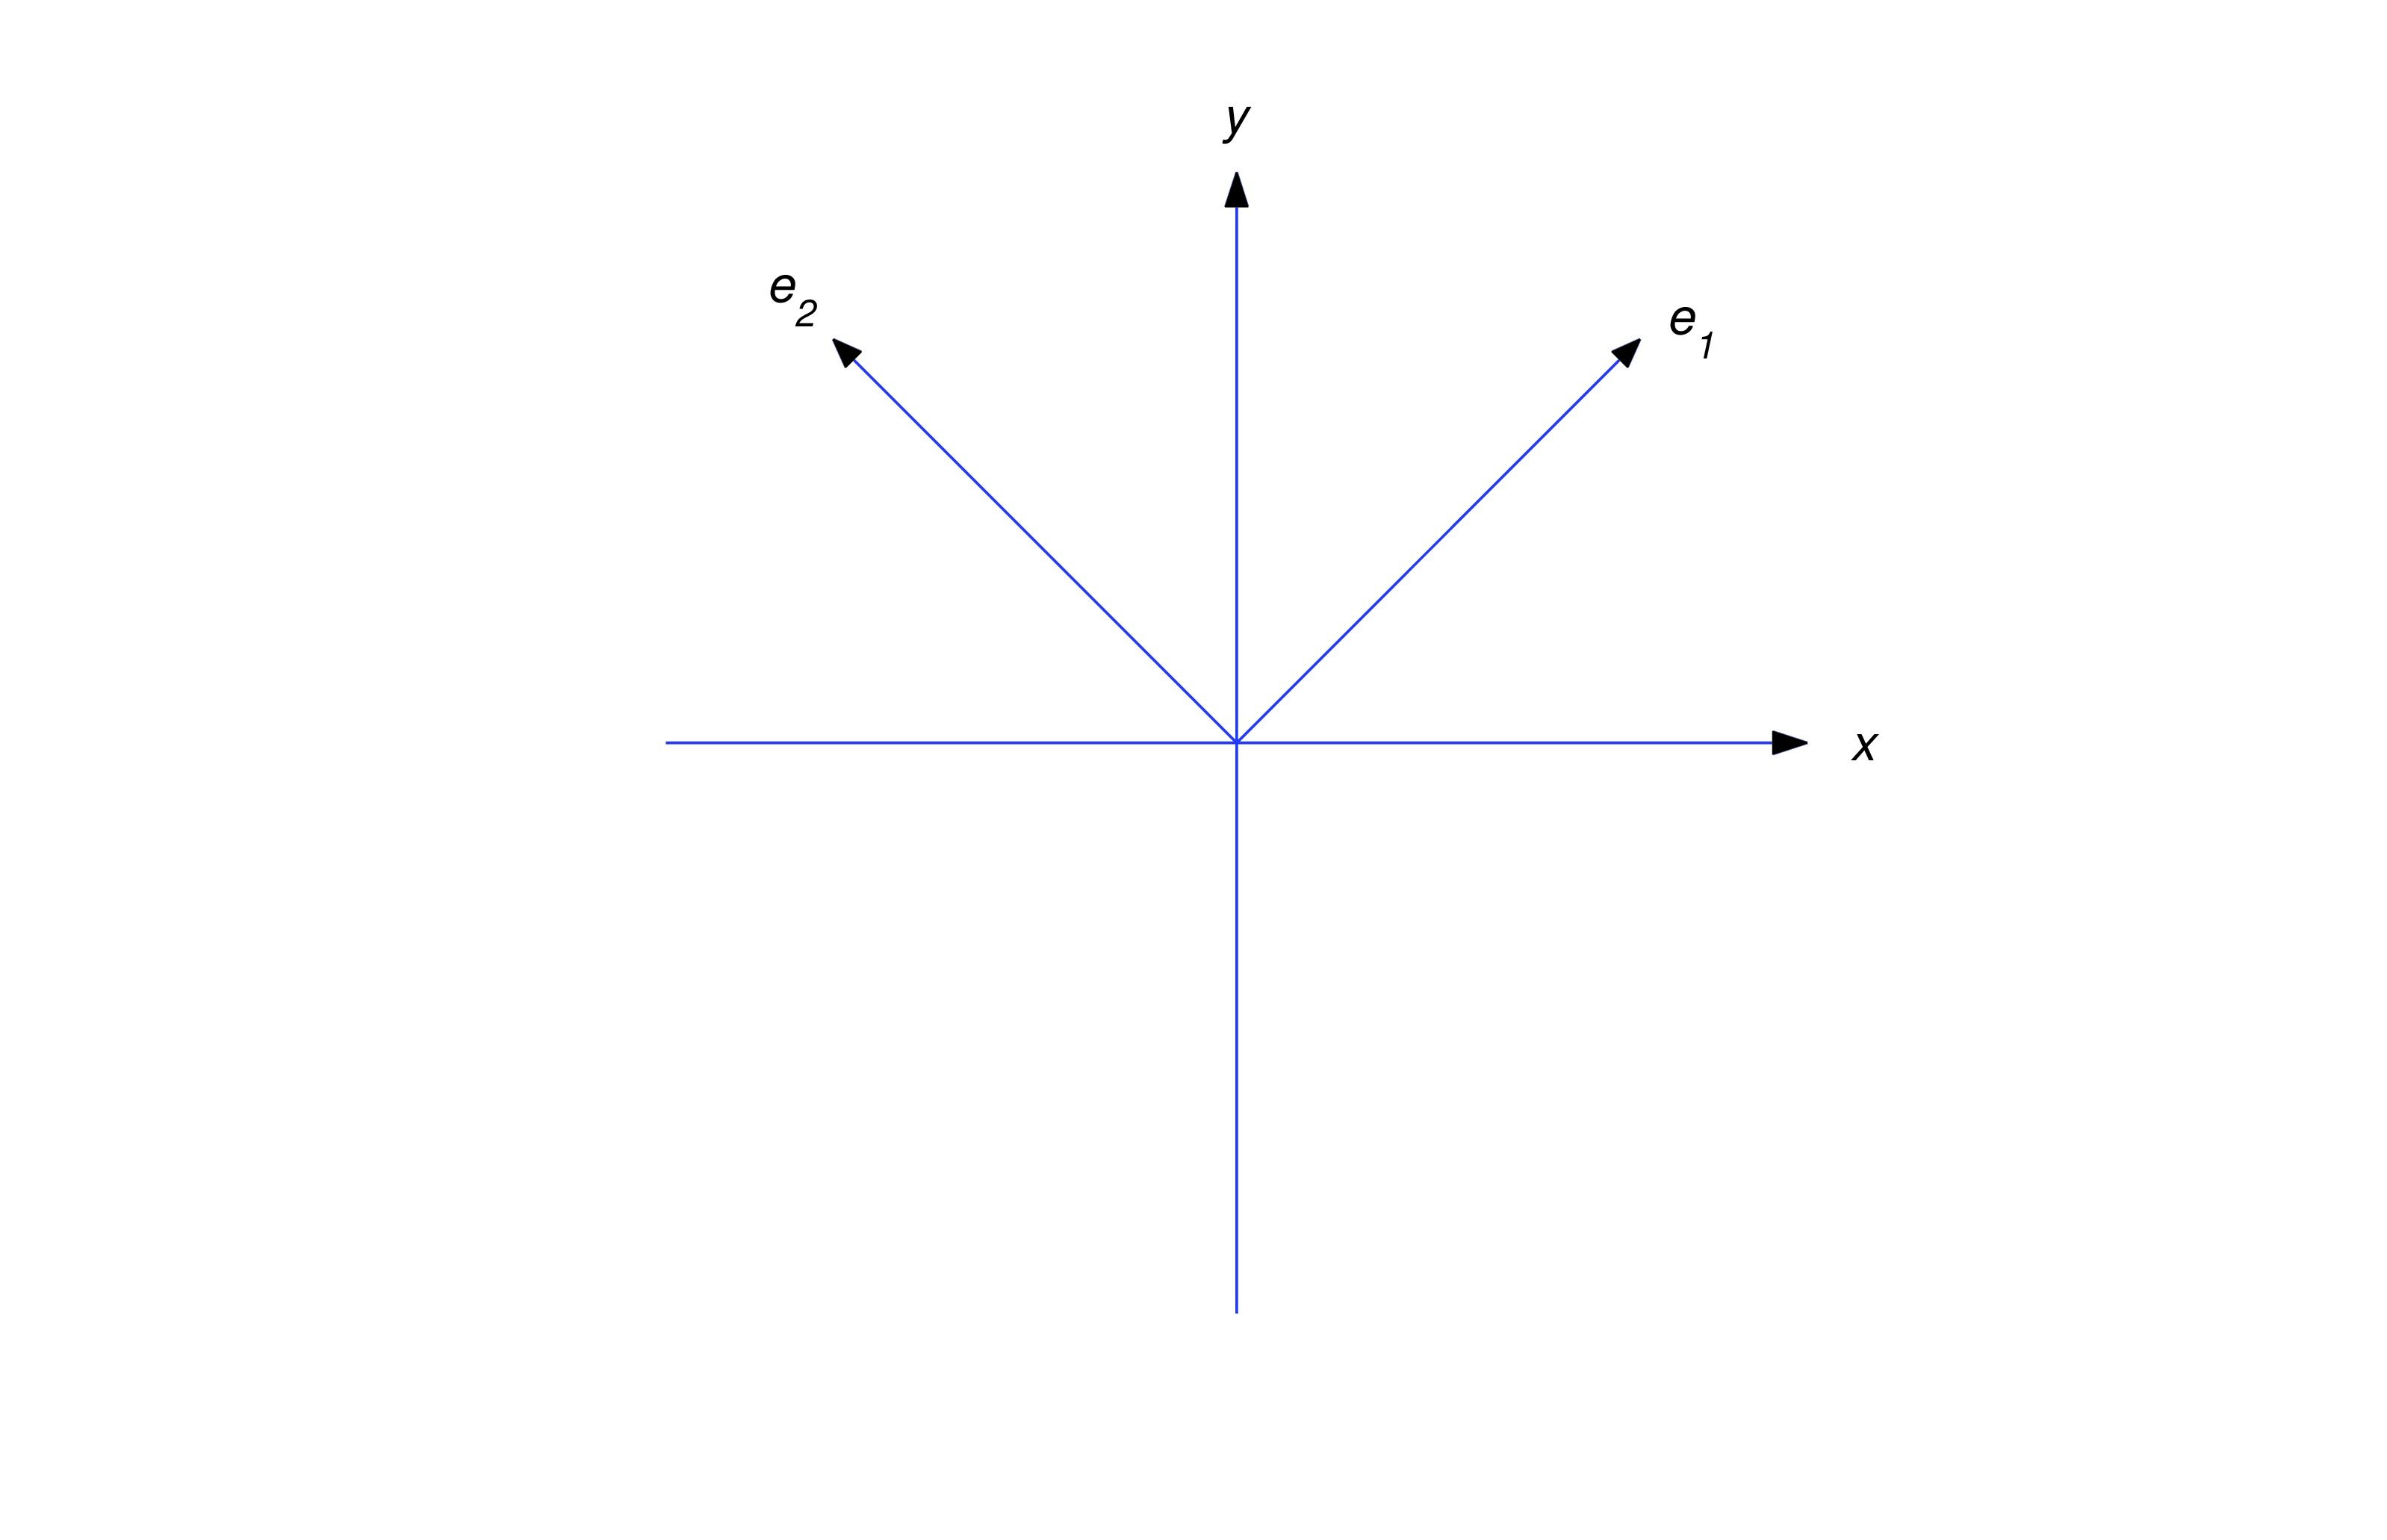
\includegraphics[height=1.5in]{fig060402.jpg}
 \end{image}

Moreover,
\begin{equation} \label{eq:6.4.3}
\frac{d\vec{e}_1}{d\theta}=\vec{e}_2,\quad
\frac{d\vec{e}_2}{d\theta}=-\vec{e}_1,
\end{equation}
and
$$
\vec{e}_1\cdot\vec{e}_2=\cos\theta(-\sin\theta)+\sin\theta\cos\theta=0,
$$
so $\vec{e}_1$ and $\vec{e}_2$ are  perpendicular.
Recalling that the single prime $(')$ stands for differentiation with
respect to
$t$, we see from \eqref{eq:6.4.3}  and the chain rule that
\begin{equation} \label{eq:6.4.4}
\vec{e}_1'=\theta'\vec{e}_2\quad\mbox{and}\quad
\vec{e}_2'=-\theta'\vec{e}_1.
\end{equation}

Now we can write \eqref{eq:6.4.2} as
\begin{equation} \label{eq:6.4.5}
m(r\vec{e}_1)''=f(r)\vec{e}_1.
\end{equation}
But
$$
(r\vec{e}_1)'=r'\vec{e}_1+r\vec{e}_1'=r'\vec{e}_1+r\theta'\vec{e}_2
$$
(from \eqref{eq:6.4.4}), and
\begin{eqnarray*}
(r\vec{e}_1)''&=&(r'\vec{e}_1+r\theta'\vec{e}_2)'\\
&=&r''\vec{e}_1+r'\vec{e}_1'+(r\theta''+r'\theta')\vec{e}_2
+r\theta'\vec{e}_2'\\
&=&r''\vec{e}_1+r'\theta'\vec{e}_2+(r\theta''+r'\theta')\vec{e}_2 -r(\theta')^2\vec{e}_1\quad\mbox{(from \eqref{eq:6.4.4})}\\
&=&\left(r''-r(\theta')^2\right)\vec{e}_1+(r\theta''+2r'\theta')\vec{e}_2.
\end{eqnarray*}
Substituting this into \eqref{eq:6.4.5} yields
$$
m\left(r''-r(\theta')^2\right)\vec{e}_1+m(r\theta''+2r'\theta')\vec{e}_2=f(r)\vec{e}_1.
$$
By equating the coefficients of $\vec{e}_1$ and $\vec{e}_2$ on the
two sides of this equation we see that
\begin{equation} \label{eq:6.4.6}
m\left(r''-r(\theta')^2\right)=f(r)
\end{equation}
and
$$
r\theta''+2r'\theta'=0.
$$
Multiplying the last equation by $r$ yields
$$
r^2\theta''+2rr'\theta'=(r^2\theta')'=0,
$$
so
\begin{equation} \label{eq:6.4.7}
r^2\theta'=h,
\end{equation}
where $h$ is a constant that we can write in terms of the initial
conditions as
$$
h=r^2(0)\theta'(0).
$$
Since the initial position and velocity vectors are
$$
 r(0)\vec{e}_1(0)\quad\mbox{and}\quad
r'(0)\vec{e}_1(0)+r(0)\theta'(0)\vec{e}_2(0),
$$
our assumption that these two vectors are not parallel implies that
$\theta'(0)\neq 0$, so $h\neq 0$.





Now let $u=1/r$.
Then  $u^2=\theta'/h$ (from \eqref{eq:6.4.7}) and
$$
r'=-\frac{u'}{u^2}=-h\left(\frac{u'}{\theta'}\right),
$$
which implies that
\begin{equation} \label{eq:6.4.8}
r'=-h\frac{du}{d\theta},
\end{equation}
since
$$
\frac{u'}{\theta'}=\frac{du/dt}{d\theta/dt}=\frac{du}{d\theta}.
$$
Differentiating \eqref{eq:6.4.8} with respect to $t$ yields
$$
r''=-h\frac{d}{dt}\left(\frac{du}{d\theta}\right)
=-h\frac{d^2u}{d\theta^2}\theta',
$$
which implies that
$$
r''=-h^2u^2\frac{d^2u}{d\theta^2}
\quad\mbox{since}\quad \theta'=hu^2.
$$
Substituting from these equalities into
\eqref{eq:6.4.6} and recalling that $r=1/u$ yields
$$
-m\left(h^2u^2\frac{d^2u}{d\theta^2}+\frac{1}{u}h^2u^4\right)
=f(1/u),
$$
and dividing through by $-mh^2u^2$ yields \eqref{eq:6.4.1}.


Eqn.~\eqref{eq:6.4.7} has the following geometrical interpretation, which
is known as
\href{http://www-history.mcs.st-and.ac.uk/Mathematicians/Kepler.html}{Kepler's Second Law}.

\begin{theorem}\label{thmtype:6.4.1}
 The position vector
 of an object moving under a central force
sweeps out equal areas in equal times; more precisely, if
$\theta(t_1)\leq\theta(t_2)$ then the (signed) area of the sector
$$
\{(x,y)=(r\cos\theta,r\sin\theta)  :  0\leq r\leq r(\theta),
\theta(t_1)\leq\theta(t_2)\}
$$
(see the figure below) is given by
$$
A=\frac{h(t_2-t_1)}{2},
$$
where $h=r^2\theta',$ which we have shown to be constant.
\end{theorem}

\begin{image}
 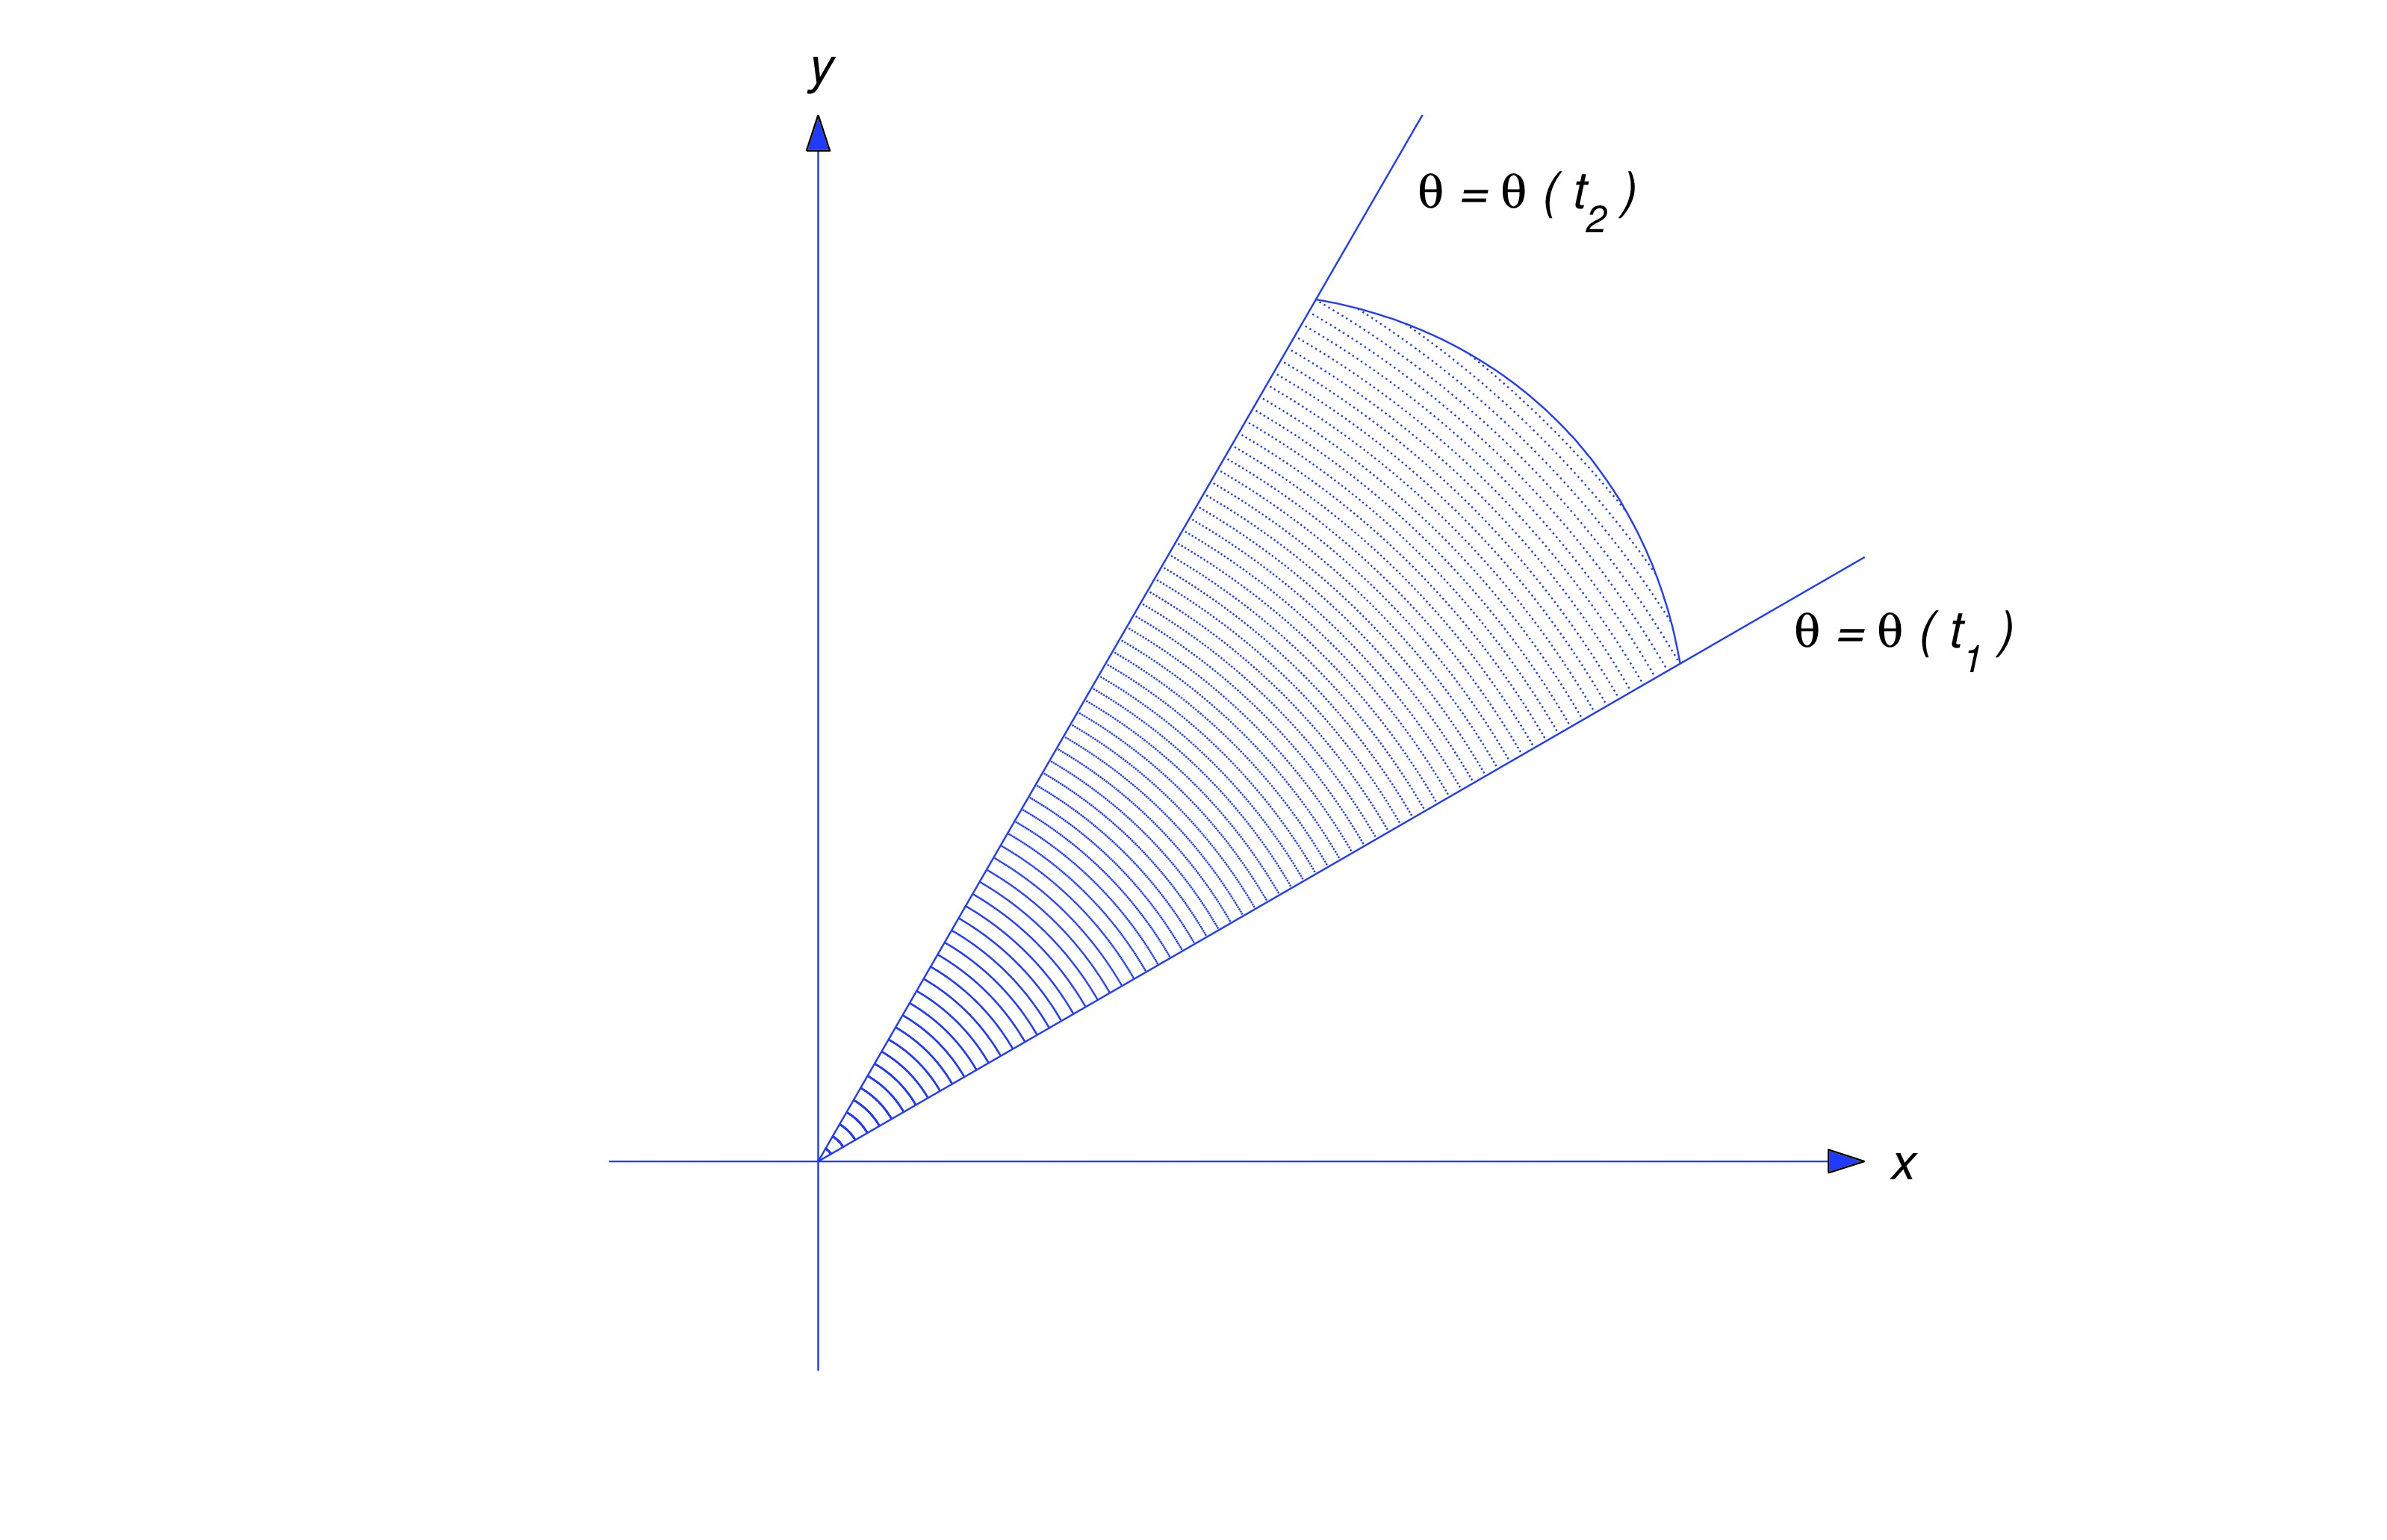
\includegraphics[height=1.5in]{fig060403.jpg}
 \end{image}

\begin{proof}  Recall from calculus that the area of the shaded sector
in the figure is
$$
A=\frac{1}{2}\int_{\theta(t_1)}^{\theta(t_2)} r^2(\theta)\,d\theta,
$$
where $r=r(\theta)$ is the polar representation of the orbit.
Making the change of variable $\theta=\theta(t)$ yields
\begin{equation} \label{eq:6.4.9}
A=\frac{1}{2}\int_{t_1}^{t_2} r^2(\theta(t))\theta'(t)\,dt.
\end{equation}
 But
\eqref{eq:6.4.7}  and \eqref{eq:6.4.9} imply that
$$
A=\frac{1}{2}\int_{t_1}^{t_2} h\,dt=\frac{h(t_2-t_1)}{2},
$$
which completes the proof.
\end{proof}

\subsection*{Motion Under an Inverse Square Law Force}

In the special case where
 $f(r)=-mk/r^2=-mku^2$, so $\vec{F}$  can be interpreted
as a gravitational force, \eqref{eq:6.4.1}  becomes
\begin{equation} \label{eq:6.4.10}
 \frac{d^2u}{d\theta^2}+u=\frac{k}{h^2}.
\end{equation}
The general solution of the complementary equation
$$
 \frac{d^2u}{d\theta^2}+u=0
$$
can be written in amplitude--phase form as
$$
u=A\cos(\theta-\phi),
$$
where $A\ge0$ and $\phi$ is a phase angle.
Since $u_p=k/h^2$ is a particular solution of \eqref{eq:6.4.10},
the general solution of \eqref{eq:6.4.10} is
$$
u=A\cos(\theta-\phi)+\frac{k}{h^2};
$$
hence, the orbit is given by
$$
r=\left(A\cos(\theta-\phi)+\frac{k}{h^2}\right)^{-1},
$$
which we rewrite as
\begin{equation} \label{eq:6.4.11}
r=\frac{\rho}{1+e\cos(\theta-\phi)},
\end{equation}
where
$$
\rho=\frac{h^2}{k}\quad\mbox{and}\quad e=A\rho.
$$
A curve satisfying \eqref{eq:6.4.11} is a conic section with a focus at
the origin. %(Exercise~\ref{exer:6.4.1}). 
The nonnegative constant $e$ is
 the \textit{eccentricity} of the orbit, which is
an ellipse if
$e<1$
ellipse (a circle if $e=0$), a parabola if $e=1$, or a hyperbola if $e>1$.

\begin{image}
 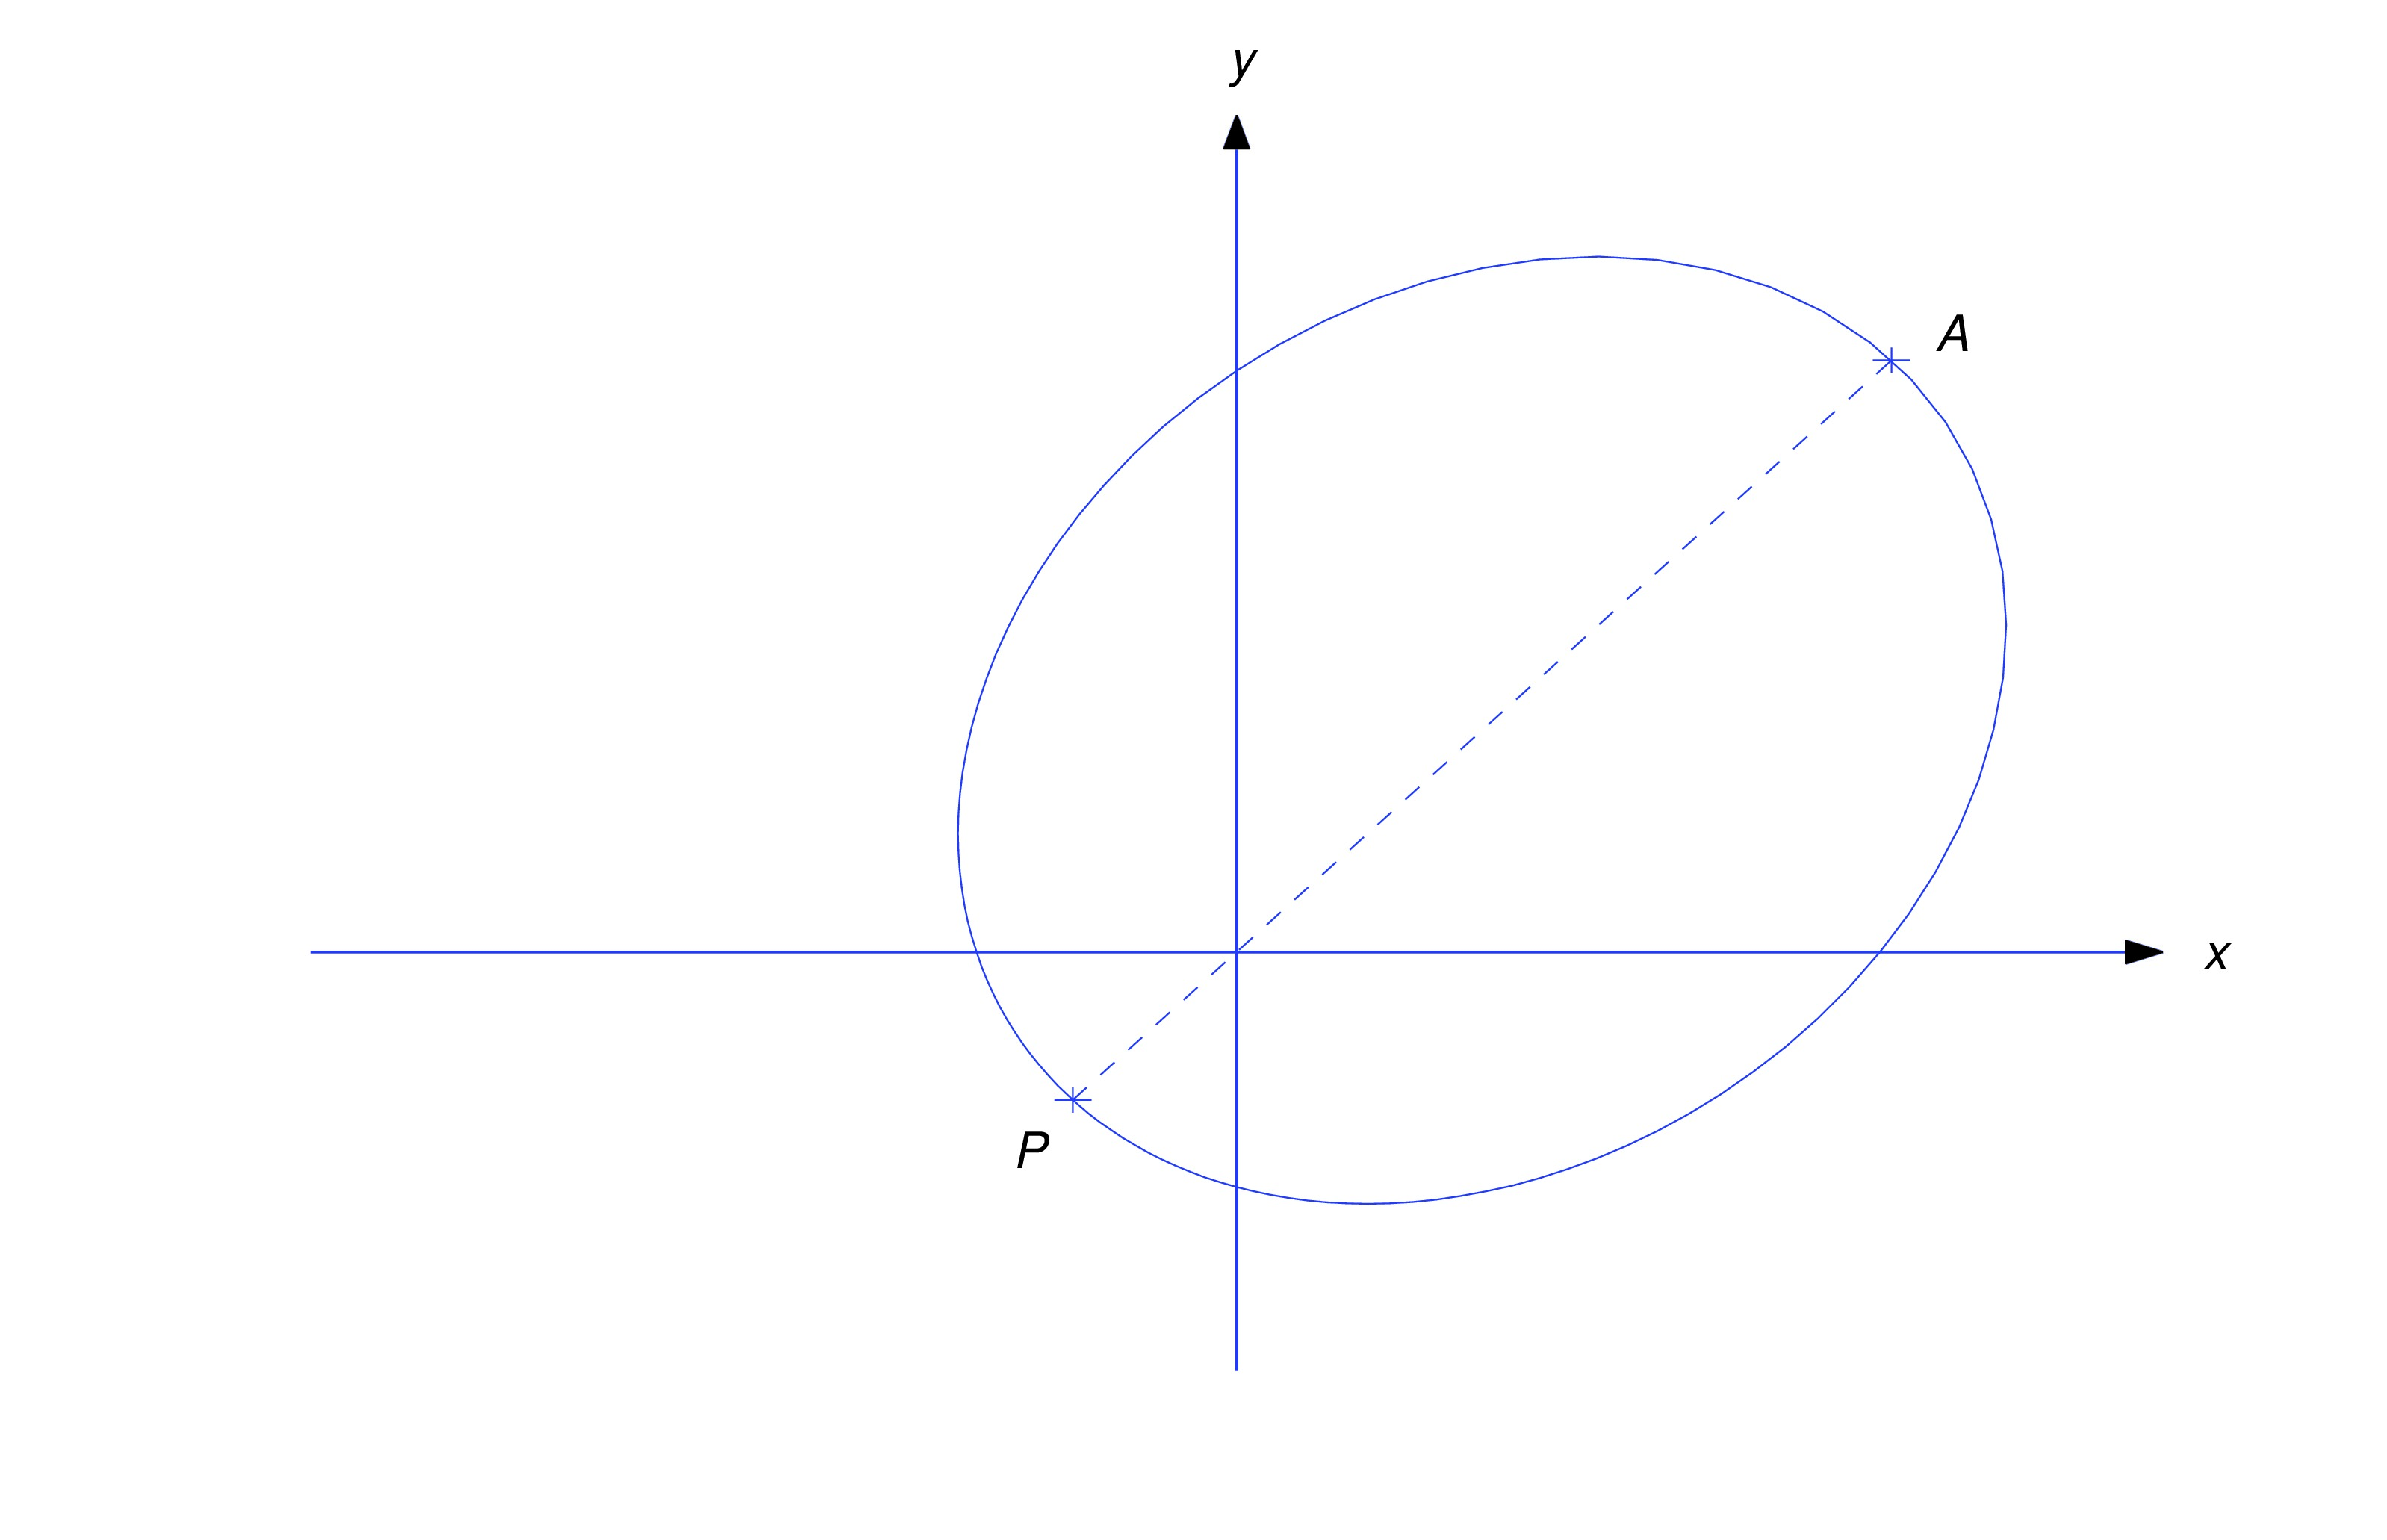
\includegraphics[height=1.5in]{fig060404.jpg}
 \end{image}

If  the orbit is an ellipse, then the minimum and maximum
values of $r$  are
\begin{eqnarray*}
r_{\min}&=&\frac{\rho}{1+e}\quad\mbox{(the \textit{perihelion
distance}, attained when
$\theta=\phi$)}  \\
 r_{\max}&=&\frac{\rho}{1-e}\quad\mbox{(the
\textit{aphelion distance}, attained when
$\theta=\phi+\pi$)}.
\end{eqnarray*}
The figure
\begin{image}
 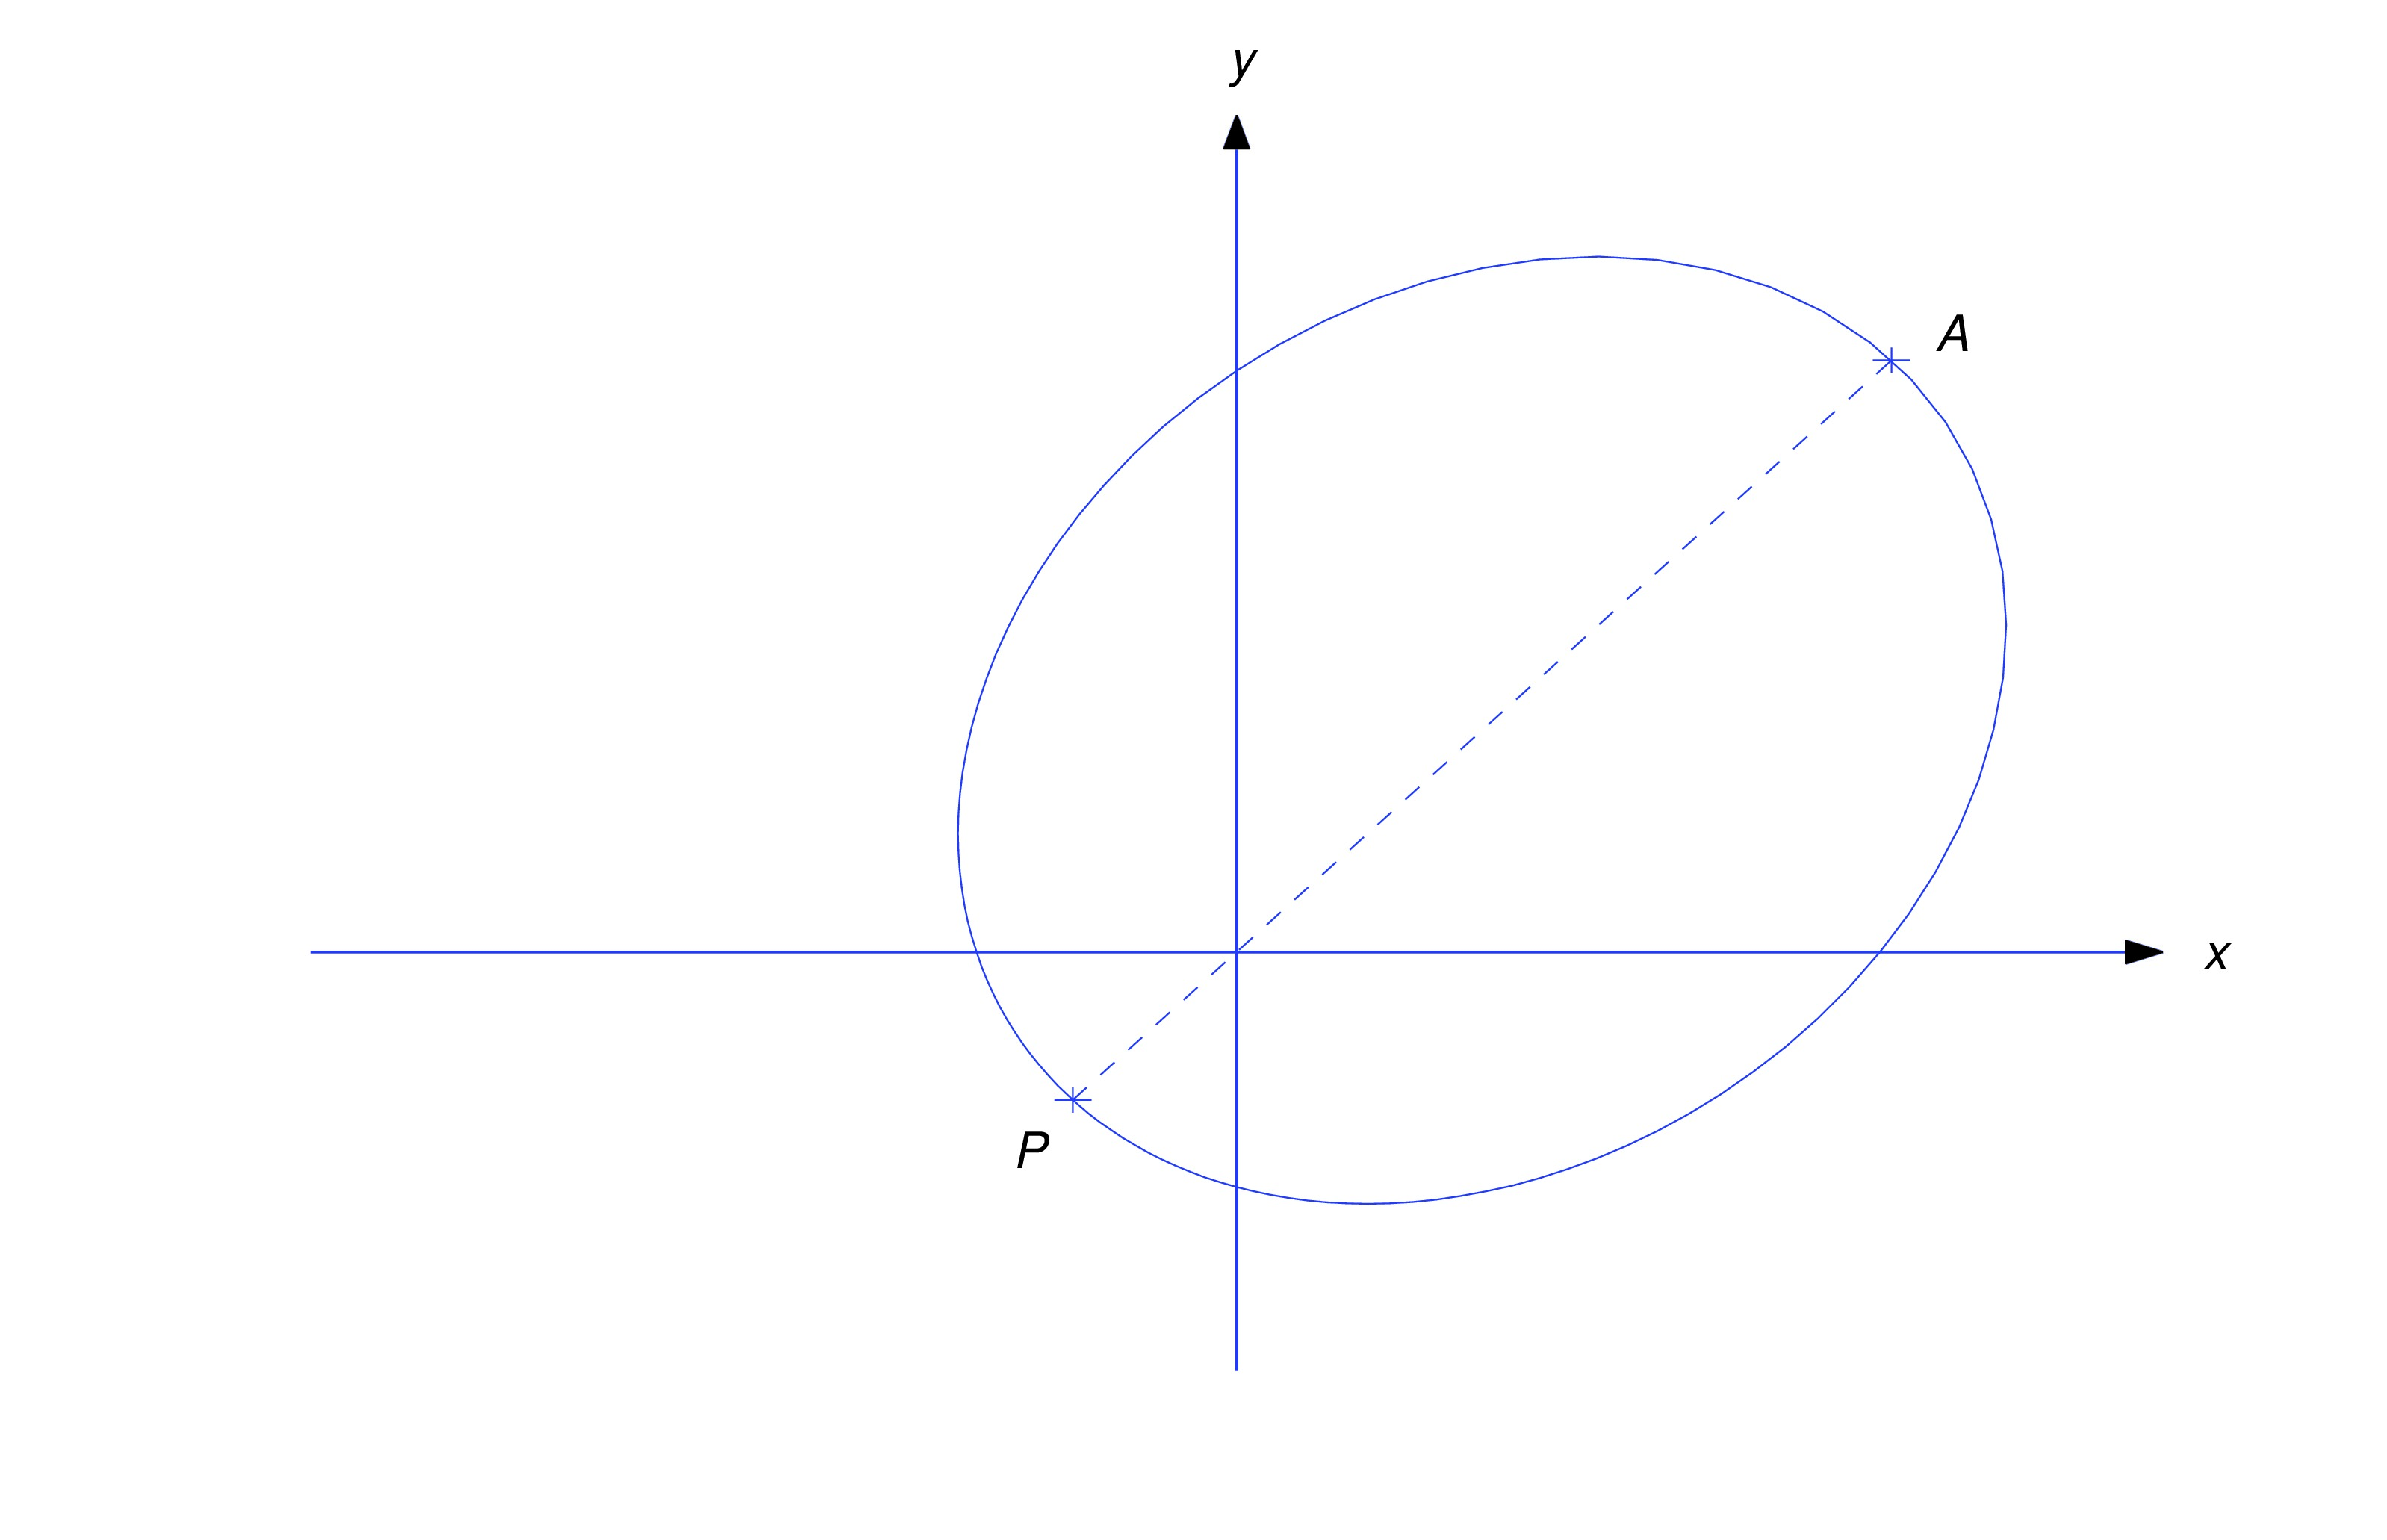
\includegraphics[height=1.5in]{fig060404.jpg}
 \end{image}

 shows a typical elliptic orbit.
The point $P$ on the orbit where $r=r_{\min}$ is the  \textit{perigee} and  the point $A$ where $r=r_{\max}$ is the \textit{apogee}.

For example, Earth's orbit around the Sun is approximately an ellipse
with $e\approx.017$, $r_{\min}\approx91\times 10^6$ miles, and
$r_{\max}\approx 95\times 10^6$ miles. Halley's comet has a very
elongated approximately elliptical orbit around the sun, with
$e\approx.967$, $r_{\min}\approx55\times10^6$ miles, and
$r_{\max}\approx33\times10^8$ miles. Some comets (the nonrecurring
type) have parabolic or hyperbolic orbits.


\section*{Text Source}
Trench, William F., "Elementary Differential Equations" (2013). Faculty Authored and Edited Books \& CDs. 8. (CC-BY-NC-SA)

\href{https://digitalcommons.trinity.edu/mono/8/}{https://digitalcommons.trinity.edu/mono/8/}


\end{document}